\documentclass[tikz,border=3.14mm]{standalone}
\begin{document}
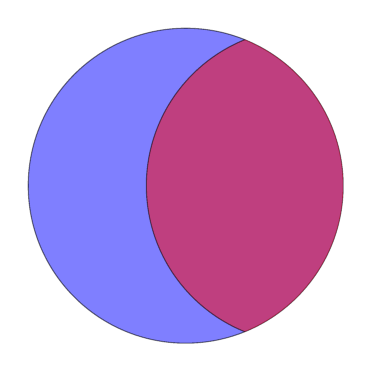
\begin{tikzpicture}

% 第一个圆
\draw[fill=blue, opacity=0.5] (0,0) circle (2);

% 第二个圆
\begin{scope}
    \clip (0,0) circle (2);  % 将第一个圆设为裁剪区域
    \draw[fill=red, opacity=0.5] (1.5, 0) circle (2);  % 绘制第二个圆,只有交集部分可见
\end{scope}

\end{tikzpicture}
\end{document}
